\documentclass[12pt]{article}
\usepackage[a4paper, total={16cm,25cm}]{geometry}
\usepackage{titlesec}
\usepackage{graphicx}
\usepackage{float}
\PassOptionsToPackage{hyphens}{url}\usepackage{hyperref}
\usepackage{fancyhdr}
\setlength{\headheight}{30pt}
\pagestyle{fancy}
\fancyhead[L]{HSI使用說明書}
\fancyhead[R]{\leftmark}
\renewcommand{\headrulewidth}{2pt}
\usepackage{amsmath}
\usepackage{latexsym}
\usepackage{multirow}
\graphicspath{ {./images/} }
\usepackage[backend=biber, citestyle=numeric, bibstyle=numeric, sorting=none]{biblatex}
\addbibresource{ref.bib}
\usepackage{mathspec}   %加這個就可以設定字體
\usepackage{xeCJK}       %讓中英文字體分開設置
\setCJKmainfont{Noto Serif CJK TC} %設定中文為系統上的字型
\newCJKfontfamily[chineseSans]\CJKsans{Noto Sans CJK TC}
\setmainfont{Roboto Serif}
\setsansfont{Roboto}
\setmonofont{Roboto Mono}
\XeTeXlinebreaklocale "zh"             %這兩行一定要加,中文才能自動換行
\XeTeXlinebreakskip = 0pt plus 1pt     %這兩行一定要加,中文才能自動換行
\renewcommand{\baselinestretch}{1.35}
\renewcommand{\figurename}{圖}
\renewcommand{\tablename}{表}
\renewcommand{\abstractname}{摘要}
\renewcommand{\contentsname}{目錄}
\renewcommand{\listtablename}{表格目錄}
%\renewcommand*{\bibfont}{\footnotesize}
\titleformat*{\section}{\Large \bfseries}
\titleformat*{\subsection}{\large \bfseries}
\titleformat*{\subsubsection}{\bfseries}

\begin{document}
    \thispagestyle{empty}\null\vspace{5cm}\noindent{\Large HyperSpectral Imaging System}\newline
    {\large 軟體操作使用說明書}\newpage
    \tableofcontents\newpage
    \section{啟動軟體}
    本軟體尚未編譯為可執行檔,請開啟並執行HIS.lvproj中的main.vi,即可啟動軟體。軟體啟動時,會自動偵測是否能成功連接iXon相機,若連接失敗,系統判定並未連接iXon,則軟體會出現訊息視窗,
    並自動進入讀取模式。
    
    一旦軟體啟動,並成功連接iXon,系統即會自動開啟iXon的TE Cooler,此時使用者即可自行輸入欲達到的溫度,待系統完成降溫且溫度穩定後,Cooler燈號才會轉為綠色。
    當系統硬體都成功連接後,軟體會自動進入影像與掃描設定的模式。此時在畫面左半側的系統控制區,多數的控制元件都會啟動,少數呈現刷白的控制元件是無法使用的。此時在影像與掃描設定模式下,
    可以對系統的影像、掃描參數進行設定,為掃描進行準備。

    同時,在畫面的右半側,共計有四個顯示螢幕,是軟體的影像資料檢索介面。該介面此時也是處於啟動狀態,能夠幫助使用者檢視當前設定下的影像資料。
    \begin{figure}[h]
        \centering
        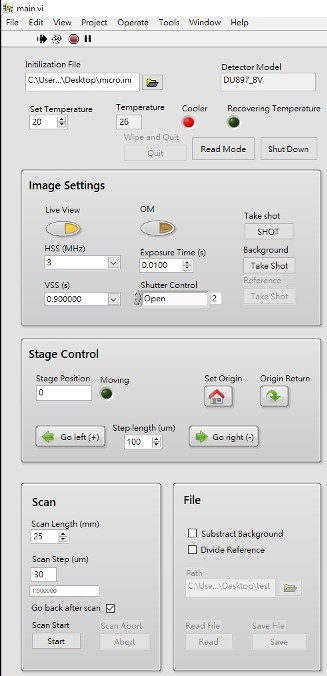
\includegraphics[width=0.33\linewidth]{settingPanel.jpeg}
        \caption{系統控制區。}
    \end{figure}
    \begin{figure}[h]
        \centering
        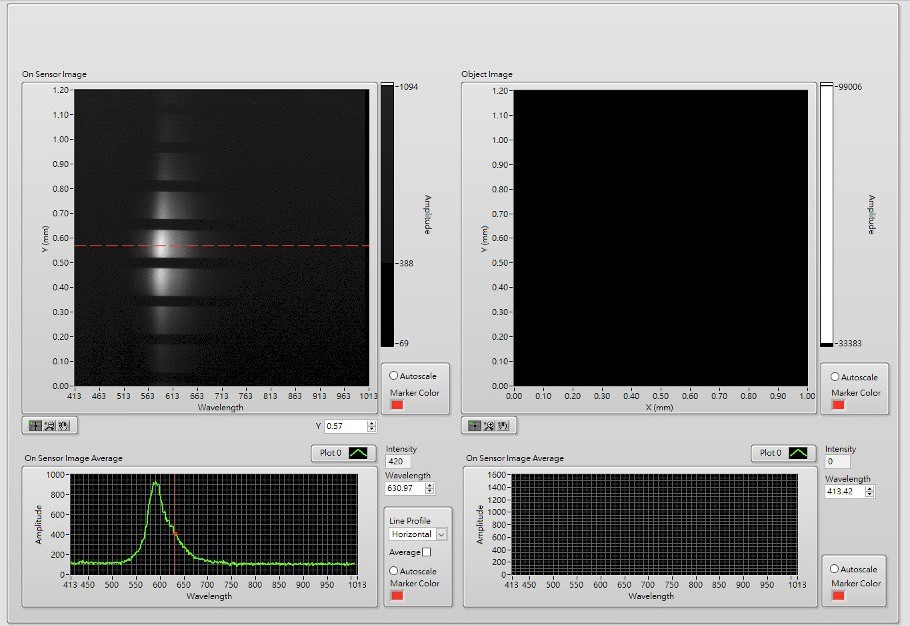
\includegraphics[width=0.75\linewidth]{browsePanel.jpeg}
        \caption{影像資料檢索介面。}
    \end{figure}

    \section{系統控制區}
    \subsection{啟動與模式控制區}
    在本區中選取系統起始參數檔(init file),一般來說使用者不需特別理會起始參數檔。若要切換起始參數檔,必須將軟體關閉後,重新指定參數檔路徑,再開啟軟體。

    若系統啟動後成功連接iXon,本區也會顯示出iXon的型號。同時,使用者可以在set temperature處設定欲使sensor達到的降溫目標,一旁的temperature則會顯示出目前的溫度。等到降溫完成且溫度穩定後,cooler status燈號才會轉為綠色。
    \footnote{請參閱iXon說明書了解合適的降溫目標溫度。}

    本區最重要的為下排的三個按鍵: quit, read mode, shut down。剛啟動時quit會被關閉,無法按下。在使用者完成掃描後,該按鍵可以讓使用者退出瀏覽模式並回到影像與掃描設定模式。
    任何時候若按下read mode,系統會直接進入讀取模式,方便使用者在只需要讀取檔案時使用。任何時候按下shut down,則會將系統關閉。請注意,關閉系統時軟體會先關閉iXon cooler,直到溫度
    回到0度c以上後,才會完全關閉系統。
    \subsection{Image Settings影像設定區}
    使用者可以在此區已各個選單調整以下影像參數:
    \begin{itemize}
        \item HSS: (Horizontal shift speed)代表的是iXon sensor橫向的讀取速度,單位為MHz,較慢的設定會等比例的加長掃描時間,一般來說將設定維持在3MHz即可。\footnote{請參閱iXon說明書了解何時須使用其他值。}
        \item VSS: (Vertical shift speed)代表的是iXon sensor直向的讀取速度,在某些情形下該參數設定較慢(如0.9s)會讓影像品質變好,不過liveview時將此設定為較快的值會有效增進frame rate。
        \item Gain: 從此下單選單選取增益。可用的增益選項是由iXon相機所決定的。增益的模式則是由init檔所決定。
        \item Exposure Time: iXon的曝光時間。
        \item Shutter Control: 開啟或關閉iXon內建的快門。請參閱iXon說明書了解其他快門模式。請先將快門開啟再開始掃描,勿使用自動快門模式。
    \end{itemize}
    另外,使用者可以在此區進行以下單張影像的擷取:
    \begin{itemize}
        \item Take Shot: 以當前的影像參數擷取一張照片,並顯示於影像資料檢索區的右側大螢幕。
        \item Background: 按下後,系統會關閉快門,以當前的影像參數擷取一張照片,並顯示於影像資料檢索區的右側大螢幕。該張影像將儲存於記憶體中,掃描結束後會用於三維影像資料的背景雜訊移除,請參閱節\ref{sec: bkg/ref}。
        \item Reference: 按下後,系統會開啟快門,以當前的影像參數擷取一張照片,並顯示於影像資料檢索區的右側大螢幕。該張影像將儲存於記憶體中,掃描結束後會用於三維影像資料的反射率計算,請參閱節\ref{sec: bkg/ref}。
    \end{itemize}

    該區有兩個重要按鍵,首先是liveview,按下後會亮起橘黃色燈號,表示目前正在實時顯示iXon sensor上的畫面,該畫面會呈現在影像資料檢索介面的左側大螢幕上。liveview時所採用的影像參數,就是當前該區所設定的參數。
    再按一次liveview鍵,liveview就會停止同時案件的燈號也會熄滅。
    \subsubsection{OM影像}
    另一個按鍵是OM,按下後同樣會亮起燈號,並在影像資料檢索介面的右側開啟一個OM顯示幕,以方便使用者觀測樣品的實際樣貌。OM畫面上的兩條白色橫虛線,標示出線光譜儀入射狹縫的視野上下界,
    而中間的垂直白色虛線,則是標示出目前入射狹縫所觀測的位置。
    
    此時OM已在進行liveview,該介面上另有OM liveview影像參數的設定選單,分別是感光度ISO與曝光時間Exposure Time,同時亦會有ROI掃描的相關控制介面出現,請參閱節\ref{sec: roi scan}。
    \begin{figure}[h]
        \centering
        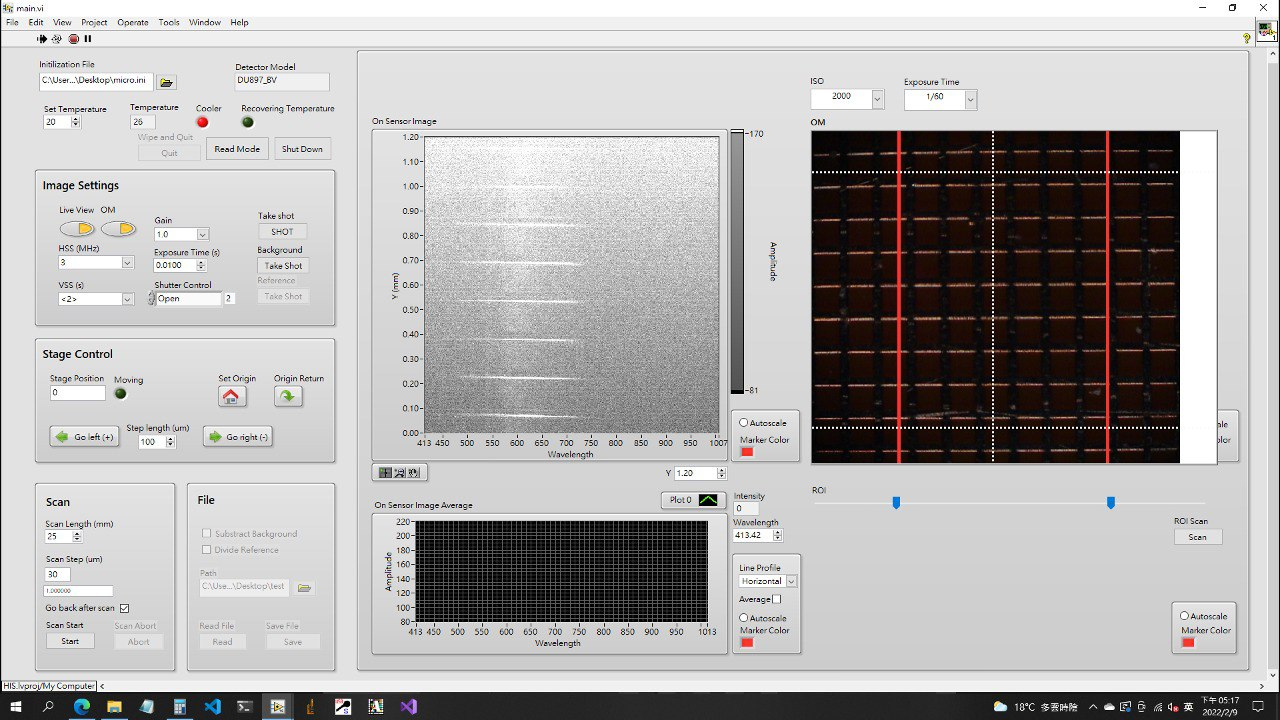
\includegraphics[width=\linewidth]{roi.jpeg}
        \caption{OM與iXon同時liveview畫面。}
        \label{fig: liveview}
    \end{figure}

    \subsection{Stage Control載台控制區}
    \subsection{Scan掃描設定區}
    \subsection{Data資料檢索區}
    \subsection{ROI掃描}\label{sec: roi scan}
    \section{影像檢索工具}
    \section{掃描}
    請先將快門開啟再開始掃描,勿使用自動快門模式。
    \section{瀏覽與存檔}
    \subsection{背景與參考光譜}\label{sec: bkg/ref}
    \subsection{讀檔}

\end{document}